\section{Results}
In the figures below, figure \ref{fig:hair}-\ref{fig:flag4}, some scenes are shown of the final results.

\begin{figure}[H]
\centering
\begin{minipage}[t]{.40\textwidth}
  \centering
  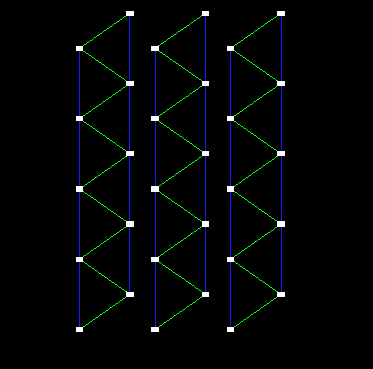
\includegraphics[height=5cm]{img/resulthair.png}
  \captionof{figure}{Start position of hair}
  \label{fig:hair}
\end{minipage}\hfill
\begin{minipage}[t]{.50\textwidth}
  \centering
  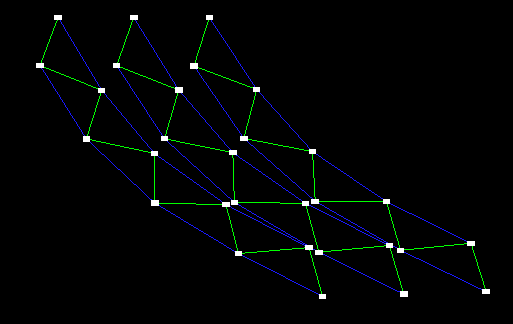
\includegraphics[height=5cm]{img/resulthair2.png}
  \captionof{figure}{Hair position after some iterations}
  \label{fig:hair2}
\end{minipage}
\end{figure}

\begin{figure}[H]
\centering
\begin{minipage}[t]{.45\textwidth}
  \centering
  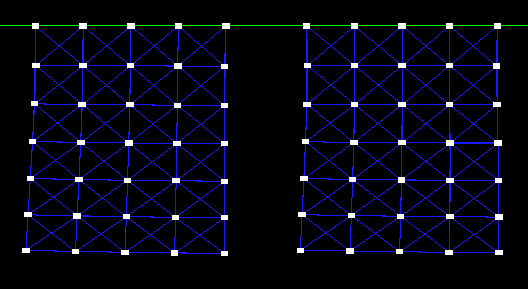
\includegraphics[height=4cm]{img/curtain.png}
  \captionof{figure}{Start position of two cloth curtains }
  \label{fig:flag3}
\end{minipage}\hfill
\begin{minipage}[t]{.45\textwidth}
  \centering
  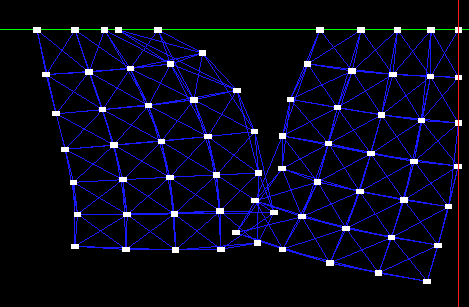
\includegraphics[height=4cm]{img/curtain2.png}
  \captionof{figure}{Two cloth curtains colliding}
  \label{fig:flag4}
\end{minipage}
\end{figure}



